The \detdeta measurement, summing over final particles of all energies, is sensitive to all aspects of the collision event, from the initial state through hadronization and final state interactions. 
Therefore, multiple event generators, \hijing, \ampt, and \epos, with different underlying physics modeling are used for comparison in this \detdeta measurement, allowing for insights into how different heavy ion collision phenomena impact \detdeta. 
For determining the MC-based correction factors used for mapping the detector-level \detdeta to the truth particle level \detdeta, the MC events are weighted to match the $z$-vertex and particle composition in data to limit model dependence in the final measurements. 

\subsection{MC Z-vertex Reweighting}
In both the data and simulation datasets, the event z-vertex is reconstructed using the MBD. 
While the z-vertex distribution in simulation is typically generated to match the z-vertex distribution in data, small discrepancies still existed between the z-vertex distribution in data and the z-vertex distribution in the simulation samples used in this analysis.
Therefore, the simulation events are reweighted to match the z-vertex distribution in data since the z-vertex distribution in data is slightly wider than the z-vertex distribution of the simulation samples. 
The z-vertex distribution in data has a mean value of 1.6 cm and width of 11.6 cm. 
The z-vertex distribution for the simulation datasets have a mean value $\sim$ 0 cm and width of 5-7 cm.
The top plots in Fig.~\ref{fig:zvtxweight} show the reconstructed z-vertex distribution using the MBD for data and three simulation samples. 
The bottom plot in Fig.~\ref{fig:zvtxweight} shows the data-over-MC z-vertex values that are used as event-by-event weights to match the z-vertex distribution to that in data. 
The MC event-level weights vary between 0.82 and 1.66 for z-vertex values in the range used for the \detdeta measurement of [-10,10] cm. 

\begin{figure}
    \centering
    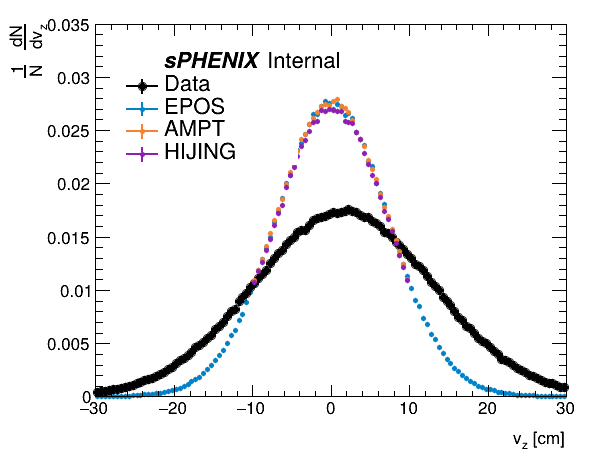
\includegraphics[width=0.48\linewidth]{detdeta/Figures/zvertex_reweighting/vz_all_runs_run24_-30_30cm.png}
    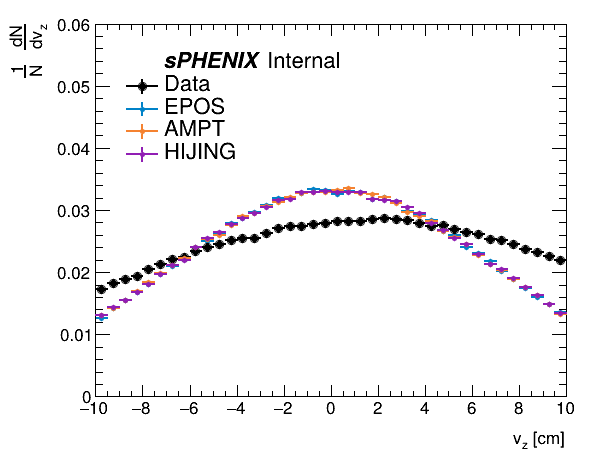
\includegraphics[width=0.48\linewidth]{detdeta/Figures/zvertex_reweighting/vz_all_runs_run24.png}
        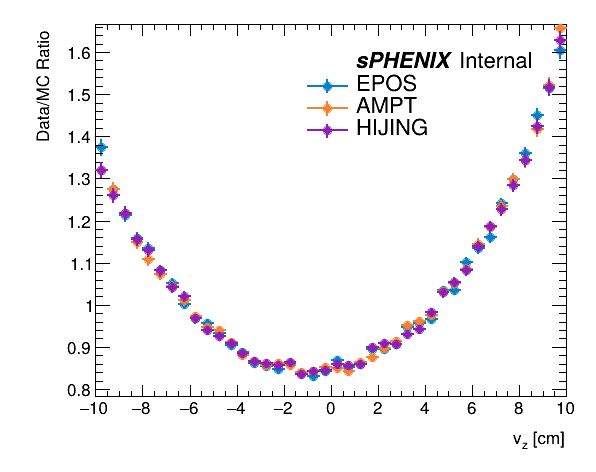
\includegraphics[width=0.48\linewidth]{detdeta/Figures/zvertex_reweighting/vz_ratio_all_runs_run24.png}
    \caption{Distributions of the z-vertex reconstructed using the MBD in data (black) and \epos (blue), \ampt (orange) and \hijing (purple) events (top) for z-vertex ranges [-30,30] cm (left) and [-10,10] cm (right), and the data-over-MC ratios (bottom).}
    \label{fig:zvtxweight}
\end{figure}

\subsection{MC Particle Composition Reweighting}
Since the \detdeta measurement is sensitive to all of the collision energy contributions, a particle composition reweighting scheme was devised to account for differences between the particle spectra produced from the event generators used in this analysis and previous measurements of identified particle spectra in Au+Au collisions at \sqsntwo.
As a first step in this reweighting procedure, the discrepancy between the final state particle spectra from the MC generators used in this analysis and previous measurements at RHIC from PHENIX and STAR was investigated~\cite{phenix_particle_spectra,star_lambda_spectra}. 
Specifically, the particle spectra of $\pi^{\pm}$, $K^{\pm}$, $p$, $\bar{p}$, $\Lambda$ and $\bar{\Lambda}$ at central rapidity ($|\eta| < 0.35$ for p, $\pi$ and K and $|\eta| < 1.0$ for $\Lambda$) as functions of transverse momentum ($p_{T}$) were studied across various centrality bins.

\subsubsection{Proton to Pion Ratios in MC Generators and Data}

Figure~\ref{fig:phenix_particle_ratios} (left) shows the proton to pion ratios as a function of particle $p_{T}$ for multiple centrality ranges from \auau collisions at 200 GeV measured by PHENIX~\cite{phenix_particle_spectra}.
Here the proton to pion ratios show the characteristic splitting across centrality bins at intermediate $p_{T}$ due to the enhanced baryon production from quark recombination and larger radial flow effects in more central collisions.
For the most central collisions (0-10\%), the proton to pion ratio peaks around 0.8 at $p_{T} \sim 2.5$ GeV, while for the most peripheral collisions (60-92\%), the ratio peaks around 0.4 at $p_{T} \sim 2$ GeV.
Figure~\ref{fig:mc_p_pi_ratio} shows the proton to pion ratio for final state truth particles from \hijing, \epos and \ampt. 

\hijing underestimates the proton to pion ratio at intermediate $p_{T}$ for most centrality bins and does not reproduce the characteristic splitting across centrality bins, with a peak value for the proton to pion ratio of around 0.4-0.5 for all centrality bins. 
\epos overestimates the proton to pion ratio at intermediate $p_{T}$ for all centrality bins, with a peak value of around 0.8 for the most centrality bins. 
However, \epos does show some small splitting effects across centrality bins, especially in the more peripheral bins of the proton to pion ratio and in the anti-proton to pion ratio.
\ampt reproduces the spread of the proton to pion ratio across centrality bins, but overestimates the centrality dependence, with a peak value of around 0.8 for the most central bin showing similar results to PHENIX, but underestimating the peak value for the more peripheral bins, with a peak value around 0.2 for the 60-92\% bin

\begin{figure}
    \centering
    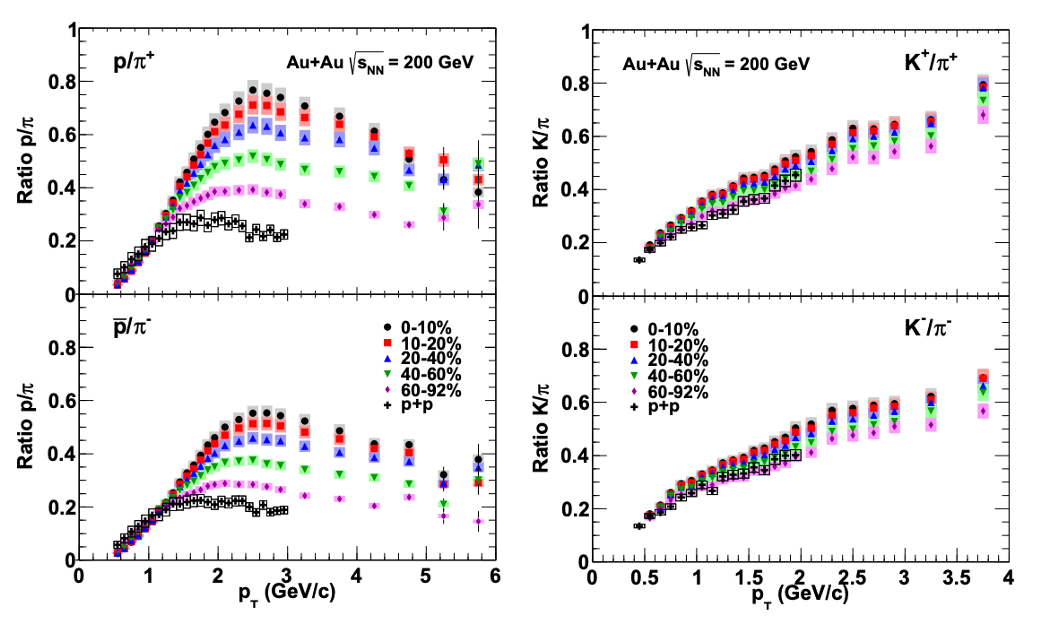
\includegraphics[width=\linewidth]{figures/chapter4/phenix_p_pi_k_pi_ratios.png}
    \caption{Proton to pion ratios (left) and kaon to pion ratios (right) as a function of particle $p_{T}$ from \auau and \pp collisions at 200 GeV measured by PHENIX. Ratios shown for \auau centrality bins $0$--$10$\% (gray), $10$--$20$\% (red), $20$--$40$\% (blue), $40$--$60$\% (green), $60$--$92$\% (pink) and inclusive \pp events (open). Reproduced from ~\cite{phenix_particle_spectra}.}
    \label{fig:phenix_particle_ratios}
\end{figure}

\begin{figure}
    \centering
    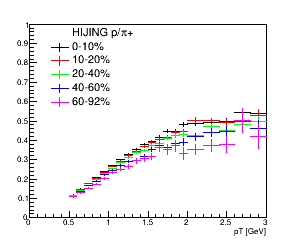
\includegraphics[width=0.48\linewidth]{detdeta/Figures/particle_comp/p_pi_ratio_hijing.png}
    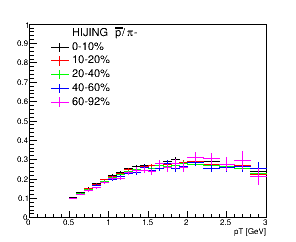
\includegraphics[width=0.48\linewidth]{detdeta/Figures/particle_comp/pbar_pi_ratio_hijing.png}
    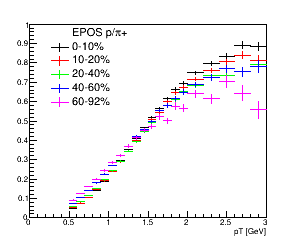
\includegraphics[width=0.48\linewidth]{detdeta/Figures/particle_comp/p_pi_ratio_epos.png}
    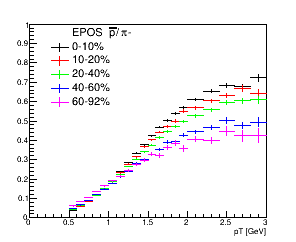
\includegraphics[width=0.48\linewidth]{detdeta/Figures/particle_comp/pbar_pi_ratio_epos.png}
    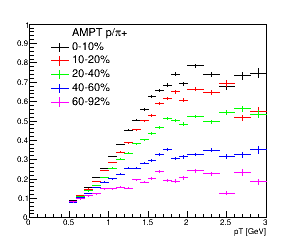
\includegraphics[width=0.48\linewidth]{detdeta/Figures/particle_comp/p_pi_ratio_ampt.png}
    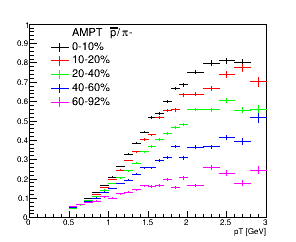
\includegraphics[width=0.48\linewidth]{detdeta/Figures/particle_comp/pbar_pi_ratio_ampt.png}
    \caption{Proton to pion ratios (left) and anti-proton to pion ratios (right) as a function of particle $p_{T}$ for generator-level particles from unweighted \hijing~(top), \ampt~(middle) and \epos~(bottom). Ratios shown for \auau centrality bins $0$--$10$\% (black), $10$--$20$\% (red), $20$--$40$\% (blue), $40$--$60$\% (green), $60$--$92$\% (pink).}
    \label{fig:mc_p_pi_ratio}
\end{figure}

\subsubsection{Kaon to Pion Ratios in MC Generators and Data}

Figure~\ref{fig:phenix_particle_ratios} (right) shows the kaon to pion ratios as a function of particle $p_{T}$ for multiple centrality ranges from \auau collisions at 200 GeV measured by PHENIX~\cite{phenix_particle_spectra}.
The kaon to pion ratios show a mild centrality dependence due to strangeness enhancement and larger radial flow effects in more central collisions.
Here the most central collisions (0-10\%) have a slightly higher kaon to pion ratio than the most peripheral \auau collisions (60-92\%) or \pp baseline across the full $p_{T}$ range, with a kaon to pion ratio at $p_{T} \sim 3$ GeV of 0.5 in peripheral collisions and 0.65 in central collisions.
Figure~\ref{fig:mc_k_pi_ratio} shows the kaon to pion ratio for final state truth particles from \hijing, \epos and \ampt.

\hijing underestimates the kaon to pion ratio across the full $p_{T}$ range and in all centrality bins, with a kaon to pion ratio at $p_{T} \sim 3$ GeV of around 0.3 for all centrality bins.
The kaon to pion ratios as a function of $p_{T}$ across centrality bins from \epos agrees fairly well with the PHENIX measurements, although slightly underestimates the ratio at higher $p_{T}$ in all centrality bins.
\ampt also underestimates the kaon to pion ratio across the full $p_{T}$ range and in all centrality bins, with a kaon to pion ratios at $p_{T} \sim 3$ GeV between 0.35 and 0.5. 
However, \ampt does exhibit a centrality dependence of similar scale to that seen in the PHENIX measurement.

\begin{figure}
    \centering
    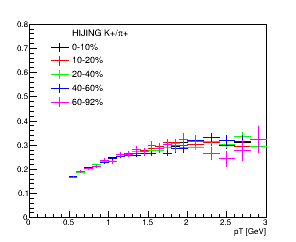
\includegraphics[width=0.48\linewidth]{detdeta/Figures/particle_comp/k_pi_ratio_hijing.png}
    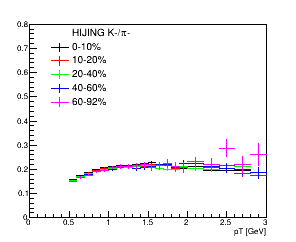
\includegraphics[width=0.48\linewidth]{detdeta/Figures/particle_comp/k-_pi_ratio_hijing.png}
    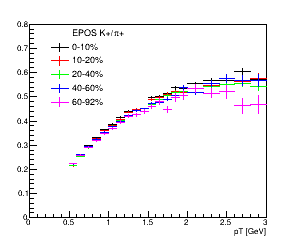
\includegraphics[width=0.48\linewidth]{detdeta/Figures/particle_comp/k+_pi_ratio_epos.png}
    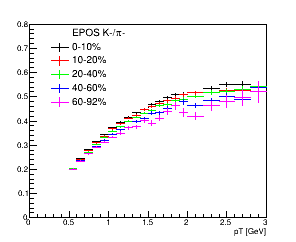
\includegraphics[width=0.48\linewidth]{detdeta/Figures/particle_comp/k-_pi_ratio_epos.png}
    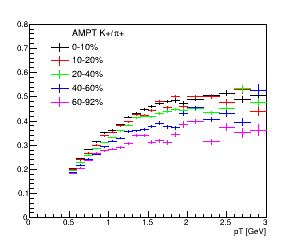
\includegraphics[width=0.48\linewidth]{detdeta/Figures/particle_comp/k+_pi_ratio_ampt.png}
    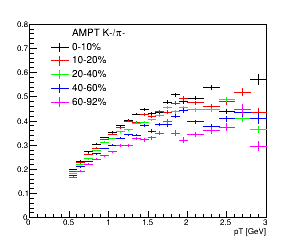
\includegraphics[width=0.48\linewidth]{detdeta/Figures/particle_comp/k-_pi_ratio_ampt.png}
    \caption{Kaon to pion ratios as a function of particle $p_{T}$ for generator-level particles from unweighted \hijing~(top), \ampt~(middle) and \epos~(bottom). Ratios shown for \auau centrality bins $0$--$10$\% (black), $10$--$20$\% (red), $20$--$40$\% (blue), $40$--$60$\% (green), $60$--$92$\% (pink).}
    \label{fig:mc_k_pi_ratio}
\end{figure}

From these studies of the proton to pion and kaon to pion ratios, none of the three MC generators were found to accurately reproduce the proton, pion and kaon particle spectra differential in $p_{T}$ and centrality seen in previous RHIC measurements. 
To correct for this discrepancy in identified particle spectra between the MC generators and experimental data, a truth-level particle and calorimeter energy reweighting module was employed within the \detdeta analysis reconstruction chain. 
This module adjusted the simulation final state truth particles and resulting detector-level calorimeter energy distribution based on the particle yield spectrum obtained from previous PHENIX and STAR experiments. 

\subsubsection{Determining MC Particle Composition Reweighting Factors}

Weight factors were created for final state particles in each of the three MC generators.
Using both the final state particle spectra of the three MC generators and the measured identified particle spectra from PHENIX and STAR~\cite{phenix_particle_spectra,star_lambda_spectra}, the invariant yields of $\pi^{\pm}$, $K^{\pm}$, $p$, $\bar{p}$, $\Lambda$, and $\bar{\Lambda}$ as functions of transverse momentum ($p_{T}$) were analyzed across various centrality bins. 
The Monte Carlo particle spectrum was calculated using the same centrality binning and $\eta$ acceptance range as was used in the PHENIX and STAR measurements. 
The MC generator spectra of $\pi^{\pm}$, $K^{\pm}$, $p$, and $\bar{p}$ were then compared to PHENIX data, while $\Lambda$ and $\bar{\Lambda}$ were compared to STAR data to compute the data/MC ratios. 

PHENIX data was specifically chosen for the p, K and pion particle reweighting procedure as it was feed-down corrected for contributions from weak decays, while the STAR data included these contributions. 
As an additional check, a comparison between the previously measured pion invariant yield in STAR and PHENIX data for three separate centrality ranges was performed as pion yields should still be affected by the feed-down corrections, but less so then protons or kaons.
Since the STAR data does not include feed-down corrections it was expected that this measurement of invariant yield of pions to be slightly higher in the lower $p_{T}$ range than the pion yield from PHENIX. 
In the comparison of STAR and PHENIX pion yield in Figure~\ref{fig:star_phenix_comparison}, small differences were observed in the pion particle spectra at low $p_{T}$ ($\sim 1$ GeV) due to the different feed-down corrections; otherwise, the spectra showed good agreement.  

\begin{figure}
    \centering
    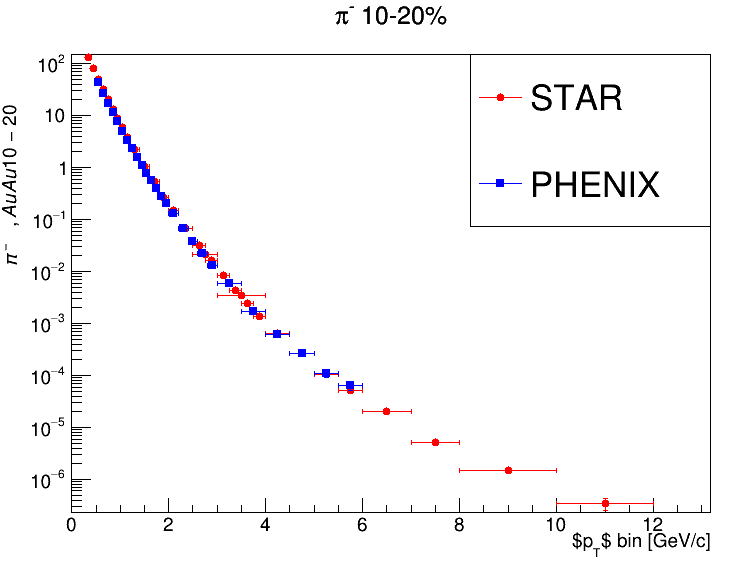
\includegraphics[width=0.48\linewidth]{detdeta/Figures/particle_comp/10-20_pions_STAR_PHENIX.png}
    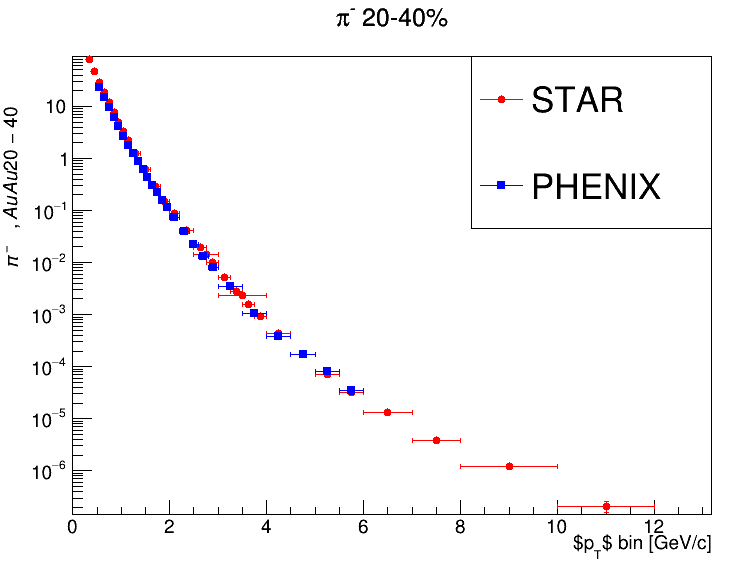
\includegraphics[width=0.48\linewidth]{detdeta/Figures/particle_comp/20-40_pions_STAR_PHENIX.png}
    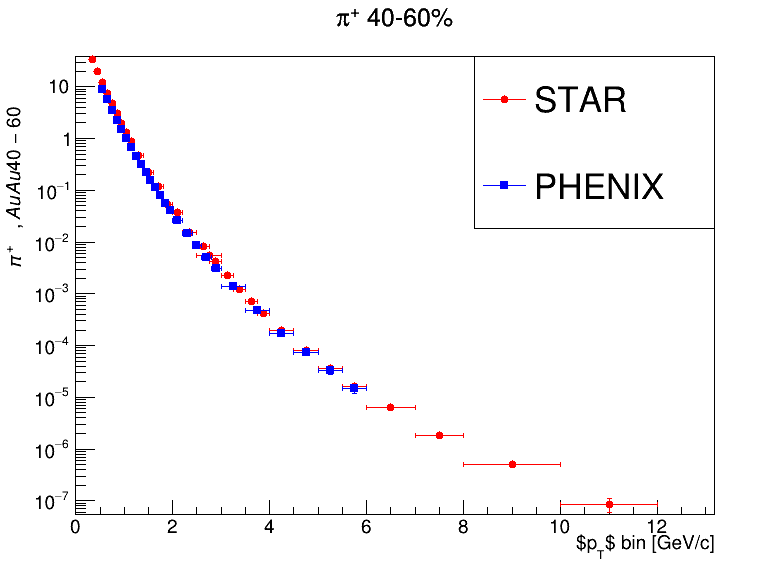
\includegraphics[width=0.48\linewidth]{detdeta/Figures/particle_comp/40-60_pions_STAR_PHENIX.png}
    \caption{Comparison of previously measured $\pi^{+}$ spectra from STAR~\cite{star_pion_p_spectra} (red) and PHENIX~\cite{phenix_particle_spectra} (blue) for centrality ranges $0$--$10$\% (top left), $20$--$40$\% (top right) and $40$--$60$\% (bottom).}
    \label{fig:star_phenix_comparison}
\end{figure}

The data/MC ratio as a function of $p_{T}$ for each centrality range was then fit with a Padé approximation of order 2/2, and this fit function was used as the reweighting factor for each specific particle. 
This is illustrated for \hijing proton and kaon reweighting factors in Fig. \ref{fig:hijing_data_mc_ratios}, where proton yield weight factors of $\sim 2$ at intermediate $p_{T}$ values can be understood to represent the inclusion of radial flow effects and enhanced baryon production.
All remaining MC generator particle composition reweighting factors used in this analysis are outlined in Appendix \ref{sec:MC_particle_ratios}. 
For neutral pions and kaons, the reweighting factor was determined as the average of the charged counterparts' reweighting factors. 
For $\Sigma$ baryons, the reweighting factor used is the same as that for $\Lambda$'s.
Finally, for baryons and anti-baryons other than $\Lambda$'s and $\Sigma$'s, the reweighting factor used is the same as p and $\bar{p}$ respectively. 

\begin{figure}
    \centering 
    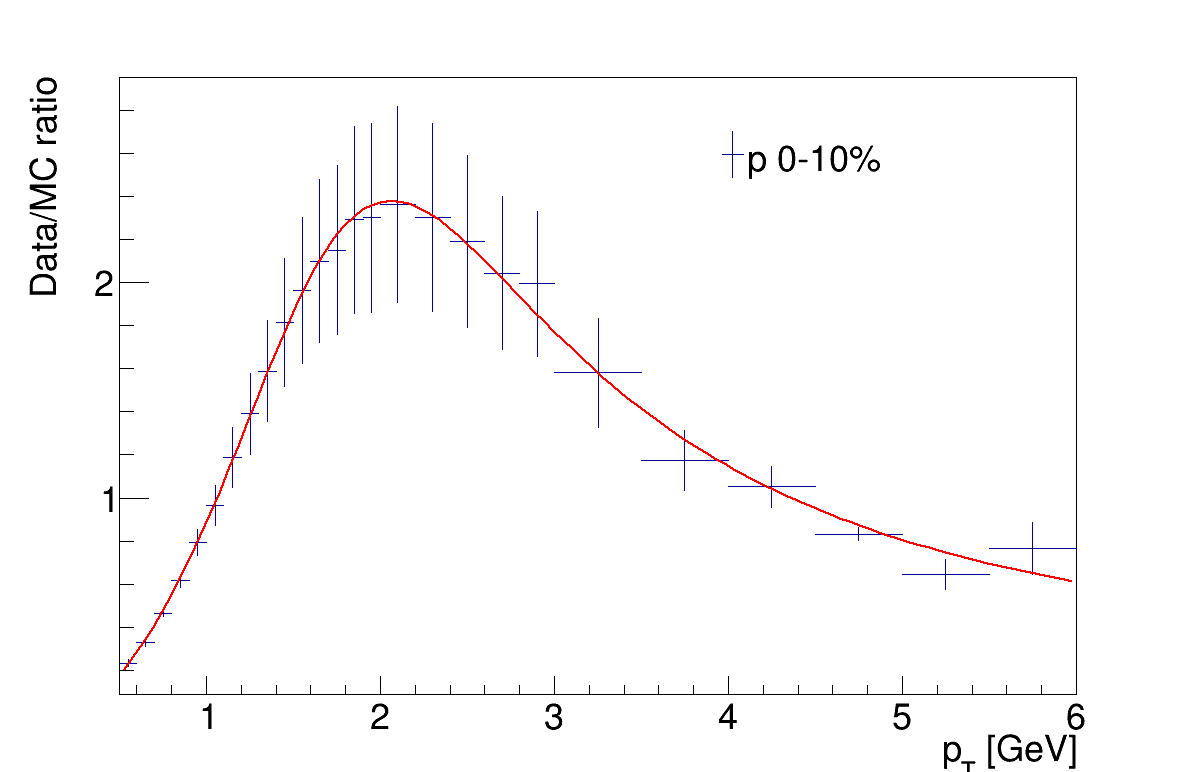
\includegraphics[width=0.48\linewidth]{detdeta/Figures/particle_reweighting_ratios/HIJING_p_0.png}
    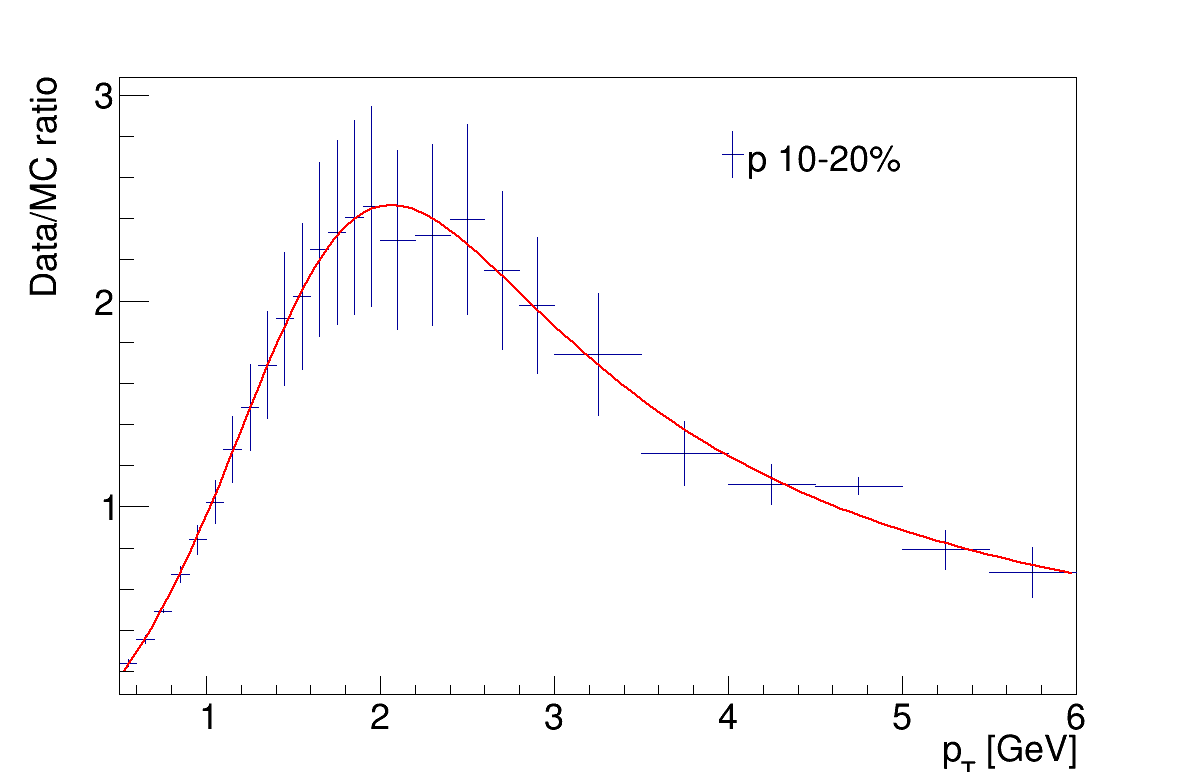
\includegraphics[width=0.48\linewidth]{detdeta/Figures/particle_reweighting_ratios/HIJING_p_1.png}
    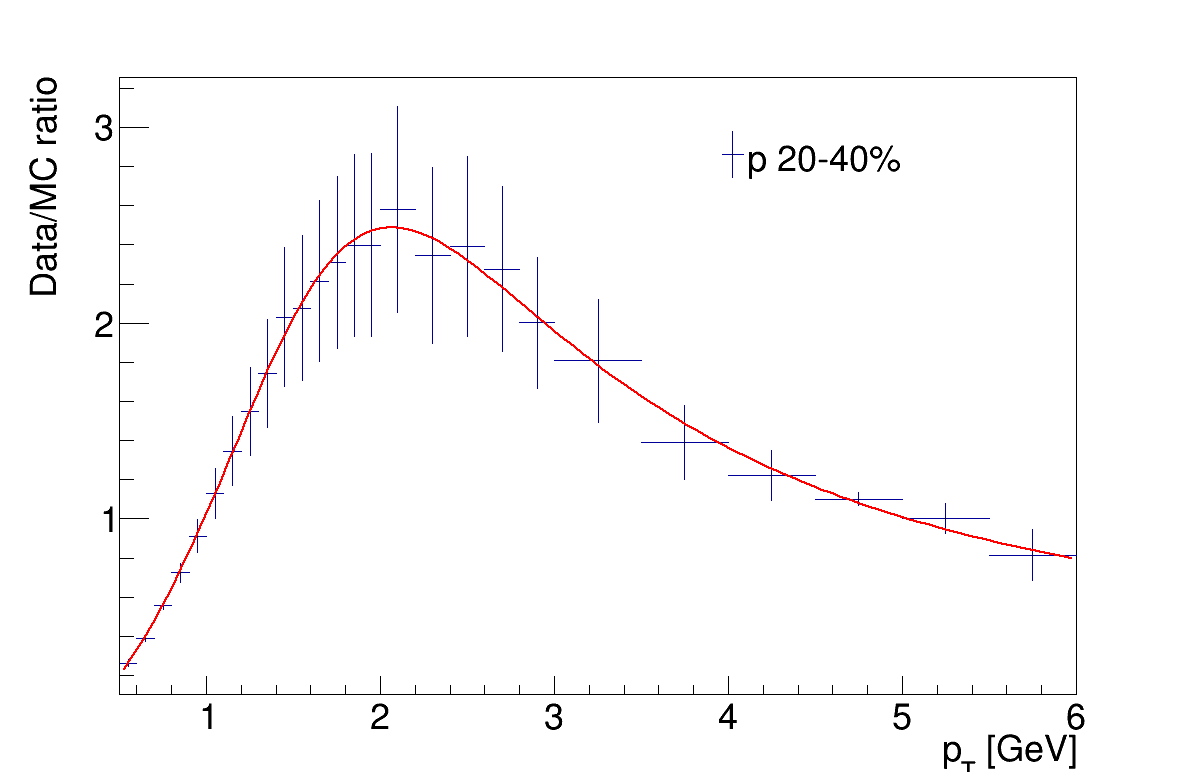
\includegraphics[width=0.48\linewidth]{detdeta/Figures/particle_reweighting_ratios/HIJING_p_2.png}
    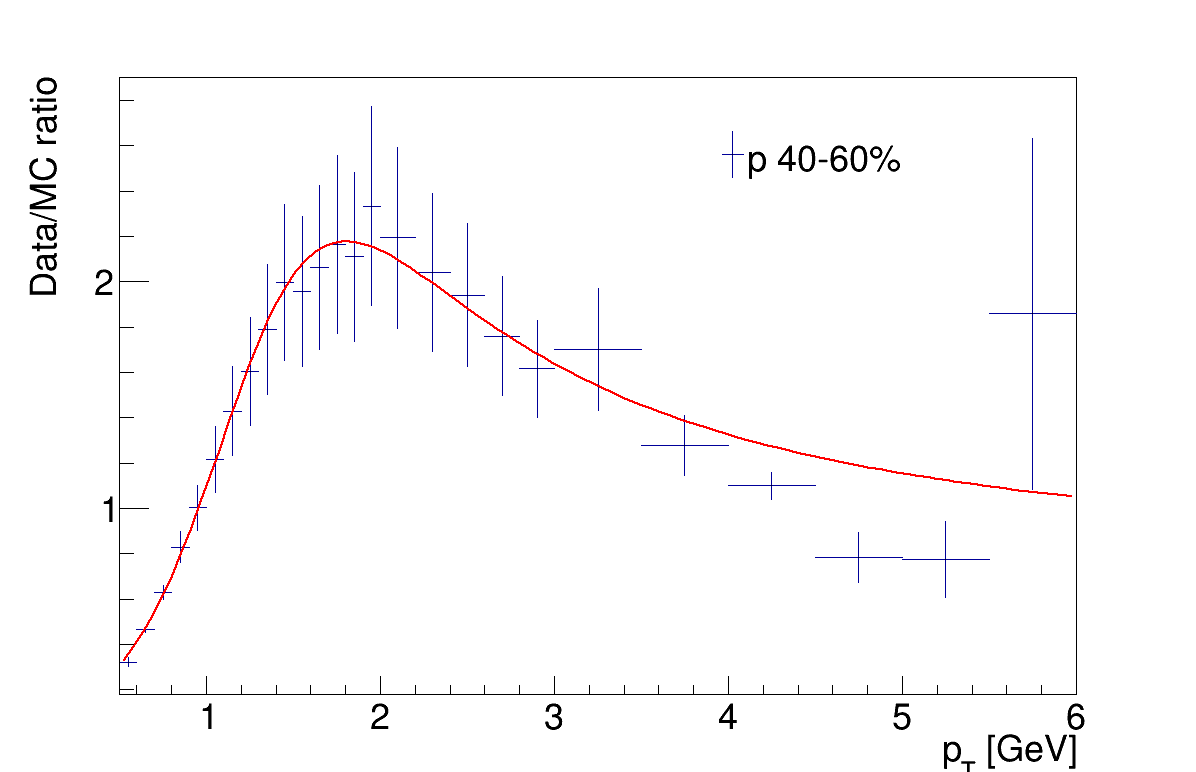
\includegraphics[width=0.48\linewidth]{detdeta/Figures/particle_reweighting_ratios/HIJING_p_3.png}
    \caption{Data to MC ratios of proton yields for \sqsntwo \auau PHENIX data \cite{phenix_particle_spectra} versus \hijing for centrality ranges $0$--$10$\% (top left), $10$--$20$\% (top right), $20$--$40$\% (bottom left) and $40$--$60$\% (bottom right).}
    \label{fig:hijing_data_mc_ratios}
\end{figure}

\subsubsection{Applying MC Particle Composition Reweighting Factors}

The reweighting factors determined from the data/MC ratios of identified particle spectra are propagated to the detector-level calorimeter towers and final state truth particles of the MC generator simulation events after running through the full \geant detector simulation.
This is afterburner style reweighting is accomplished for the detector-level calorimeter towers by first tracing back each G4Hit for each calorimeter tower in the detector to its originating final state particle. 
The reweighting factor for each hit is then calculated based on the primary parent particle's particle ID (PID), transverse momentum ($p_{T}$), and the event's centrality. 
This factor is derived from interpolating the MC/data ratios across different centrality bins as a function of $p_{T}$ and using fits like those shown in Figure~\ref{fig:hijing_data_mc_ratios} to ensure a precise adjustment of the G4Hit energy.
This same reweighting factor is then also applied to update the final state particles' four-momenta in the truth record for the truth $\ET$ calculation.

Since this approach upweights or downweights the energy of each particle as a proxy for adding or removing particles to match the particle spectra in data, this approach does not replicate the precise conditions of each individual event.
For example, this approach equates one 2 GeV $\pi$ with two 1 GeV $\pi$.
However, this reweighting method does effectively incorporate the \textit{average} energy contributions from the data into the MC simulations across a multitude of events. 
By applying these reweighting factors, the method on average adjusts the MC simulation to approach empirical data, making the particle-level average \detdeta in the simulation more representative of real-world measurements. 